%%%%%%%%%%%%%%%%%%%%%%%%%%%%%%%%%%%%%%%%%
% Large Colored Title Article
% LaTeX Template
% Version 1.1 (25/11/12)
%
% This template has been downloaded from:
% http://www.LaTeXTemplates.com
%
% Original author:
% Frits Wenneker (http://www.howtotex.com)
%
% License:
% CC BY-NC-SA 3.0 (http://creativecommons.org/licenses/by-nc-sa/3.0/)
%
%%%%%%%%%%%%%%%%%%%%%%%%%%%%%%%%%%%%%%%%%

%----------------------------------------------------------------------------------------
%	PACKAGES AND OTHER DOCUMENT CONFIGURATIONS
%----------------------------------------------------------------------------------------

\documentclass[pdftex, DIV=calc, paper=a4, fontsize=11pt]{scrartcl}	 % A4 paper and 11pt font size


\usepackage[pdftex]{graphicx}

\usepackage[scaled]{helvet}

\usepackage{lipsum} % Used for inserting dummy 'Lorem ipsum' text into the template
\usepackage[english]{babel} % English language/hyphenation
\usepackage[utf8]{inputenc}
\usepackage[T1]{fontenc}
\usepackage[protrusion=true,expansion=true]{microtype} % Better typography
\usepackage{amsmath,amsfonts,amsthm} % Math packages
\usepackage[svgnames]{xcolor} % Enabling colors by their 'svgnames'
\usepackage[hang, small,labelfont=bf,up,textfont=it,up]{caption} % Custom captions under/above floats in tables or figures
\usepackage{booktabs} % Horizontal rules in tables
\usepackage{fix-cm}	 % Custom font sizes - used for the initial letter in the document
\usepackage{hyperref}

\usepackage{sectsty} % Enables custom section titles
\allsectionsfont{\usefont{OT1}{phv}{b}{n}} % Change the font of all section commands

\usepackage{fancyhdr} % Needed to define custom headers/footers
\pagestyle{fancy} % Enables the custom headers/footers
\usepackage{lastpage} % Used to determine the number of pages in the document (for "Page X of Total")


% Headers - all currently empty
\lhead{}
\chead{}
\rhead{}

% Footers
\lfoot{}
\cfoot{}
\rfoot{\footnotesize Page \thepage\ of \pageref{LastPage}} % "Page 1 of 2"

\renewcommand{\headrulewidth}{0.0pt} % No header rule
\renewcommand{\footrulewidth}{0.4pt} % Thin footer rule

\usepackage{lettrine} % Package to accentuate the first letter of the text
\newcommand{\initial}[1]{ % Defines the command and style for the first letter
\lettrine[lines=3,lhang=0.3,nindent=0em]{
\color{DarkGray}
{\textsf{#1}}}{}}

%----------------------------------------------------------------------------------------
%	TITLE SECTION
%----------------------------------------------------------------------------------------


\usepackage[pdftex]{graphicx}
\usepackage{xcolor}
\definecolor{dark-gray-Large}{RGB}{78,79,81}
\definecolor{dark-gray}{RGB}{70,71,73}

\newcommand{\HRule}{\rule{\linewidth}{0.5mm}}

%----------------------------------------------------------------------------------------

\begin{document}

\begin{titlepage}
\begin{center}

% Upper part of the page. The '~' is needed because \\
% only works if a paragraph has started.

~\\
~\\
~\\
~\\
~\\


\includegraphics[width=0.55\textwidth]{RUheader.png}~\\[1cm]


% Title
\color{dark-gray-Large}\HRule \\[0.4cm]
{ \huge \bfseries \color{dark-gray-Large}iSchool App \\[0.4cm] }

\HRule \\[1.5cm]

% Author and supervisor
\noindent
\begin{minipage}{0.4\textwidth}
\begin{flushleft} \large
\emph{\color{dark-gray}Authors:}\\
\color{dark-gray}Björn Orri \textsc{Sæmundsson}\\
Kári Tristan \textsc{Helgason}\\
Starkaður \textsc{Hróbjartsson}\\
\end{flushleft}
\end{minipage}%
\begin{minipage}{0.4\textwidth}
\begin{flushright} \large
\emph{\color{dark-gray}Supervisor:} \\
\color{dark-gray}Hlynur \textsc{Sigþórsson}
\end{flushright}
\end{minipage}

~\\
~\\
~\\


\includegraphics[width=0.35\textwidth]{AppIcon.jpg}~\\[1cm]

\vfill

% Bottom of the page
{\large \today}

\end{center}
\end{titlepage}

\thispagestyle{fancy} % Enabling the custom headers/footers for the first page 
% Reset page count so as to not count the title page.
\setcounter{page}{1}

%----------------------------------------------------------------------------------------
%	ABSTRACT
%----------------------------------------------------------------------------------------
\section*{Abstract}
\initial{T}\textbf{he work described in this report is our solution to the problem of accessing
information from MySchool on a mobile client. This report is the product of work done on an UROP
assignment in the fall term of 2014. In this report we present a new mobile application
for viewing information from MySchool in an easy-to-use, accessible format to simplify the life
of the highly mobile student. The application is native to Apple's iOS operating system and
aims to improve upon the already available and quite popular MyRU app, which we created in the fall of 2013.}

\pagebreak

\tableofcontents

\pagebreak

%----------------------------------------------------------------------------------------
%	ARTICLE CONTENTS
%----------------------------------------------------------------------------------------

\section{Introduction}

This report details the work done by the authors in the fall term of 2014. We chose this assignment
as a UROP project, as we had previous experience and we felt it would be a valuable project,
both for us personally and potentially for Reykjavik University. The authors are students at Reykjavik University
in their last year of studies for a B.Sc. in Software engineering. Björn Orri Sæmundsson and 
Kári Tristan Helgason are the authors of a previous app for MySchool\cite{myschool}
called MyRU\cite{myru}, created in 2013. 

The problem we set out to solve is that MySchool is by no stretch of the imagination easy to use
on a mobile platform. MySchool is an ageing web service created at a time before mobile phones
reached ubiquity, and presents a user interface that requires the
user to be situated in front of a desktop computer to use. The layout of the website lends itself
poorly to the portrait screen layout of mobile phones. There is an abundance of content on the
front page, making it very hard to find what one is looking for on a smaller screen. This also
causes problems for touch interactions, as links and buttons are often small.

Writing applications that talk to MySchool would be a simple matter if it presented an API
(Application programming interface) to program against. No such API currently exists, and thus
we are forced to extract the data from the website as it is presented to a human user.

Our solution is a native iOS\cite{ios} mobile application written in Apple's new programming language Swift\cite{swift}.
Our aim with this project is making MySchool easier to access and more pleasant to use on a mobile
device.

In section \ref{sec:myru} we describe the MyRU app that iSchool replaces and explain how the new iSchool
app improves upon MyRU. Section \ref{sec:swift} briefly introduces the Swift language, explain why we chose it
and details on some of the problems we faced when developing in a language still at a beta stage. Section
\ref{sec:ischool} introduces the iSchool app and explains how it solves the problem. We outline
the architecture of the application in section \ref{sec:arch} and explain various design decisions.
In section \ref{sec:progress} we talk about how the work progressed and how much time was spent on
development. Finally in section \ref{sec:future} we propose several ideas for extending the
functionality of the app and discuss possible improvements.

\section{MyRU}
\label{sec:myru}

Björn and Kári created the MyRU app, available both for iOS and Google's Android
operating system\cite{android}, which has gained much traction among students enrolled at RU. At the time of writing 810 
and 615 students have installed the iOS and Android apps respectively. The latest available data 
from RU is from 2011, and shows 2942 students enrolled in total\cite{students}. So nearly half of students at the 
university have installed the app. This demonstrates the enormous interest that students have
in the project.
The previous version of the app did have some problems. Development was haphazard and the code was not
properly tested. There were concurrency problems and in particular a certain error would
cause the app to crash randomly. In light of the fact that the app had gained such traction we 
wanted to make sure that it would work well and reliably, in order to reflect positively on us and
the university.

MyRU was a hobby project from the start, and not initially intended for release on the App Store.
However due to interest from fellow students we decided to release it publicly.
In light of this we decided that rewriting the app in a more maintainable fashion, with proper structure and tests
would be the best way to create a long term viable solution.

\section{Swift}
\label{sec:swift}

At the WWDC\cite{wwdc} conference in June Apple surprised everyone when they announced their new programming
language Swift. Swift was designed to be a very modern programming language, and incorporates
many innovations in programming language design.

Some of the impressive features that swift offers are
\begin{description}
    \item[Functional programming style] In Swift, functions are objects just like everything else.
        This enables interesting programming patterns such as passing around callbacks. This feature
        is the defining property of many functional languages. Swift incorporates other features 
        of functional languages, such as the trio of functions \texttt{map}, \texttt{filter} and \texttt{fold}.
    \item[Immutable by default] Variables are declared with the \texttt{let} or \texttt{var}
        keywords. Variables declared with \texttt{let} are immutable. This allows the compiler to
        do all sorts of clever optimisations and allows one to detect many mistakes at compile-time.
    \item[Sensible Switch-Case] The switch statement in Swift allows programmers to pattern match on
        any value, not just integers as in many classic programming languages. This allows one 
        to write nice and terse code, that's also very fast.
    \item[Strict typing and type inference] The compiler enforces types to make errors apparent as
        soon as possible, but frees the programmer from the burden of declaring a type for every
        variable explicitly.
    \item[Powerful enums and structures] In Swift, structures and enums can have methods associated with them. In addition, any value can be associated with an enum, not just integers.
    \item[Optionals] This language feature makes it easy to implement nil checks and prevents the 
        dreaded errors that occur when nils bubble up through a program. Functions that return 
        optional types are wrapped in an Optional that contains either nil or a value. 
\end{description}

These are just a few of the improvements that Swift brings. It's also appropriate to mention the fact
that objects in Swift are reference-counted, freeing the programmer from the cognitive burden of
explicitly allocating and freeing memory, while also avoiding the runtime overhead that comes with
garbage collection. It's also compiled to native code with LLVM\cite{llvm}, and is very fast, in some cases even
faster than C, the language often regarded as the gold standard when it comes to speed.

Applications for Apple's operating systems have classically been written in the language Objective-C,
developed at NeXT in in the early 1980's.
To ease the transition to Swift Apple made sure that interoperability with existing Objective-C 
code was seamless. This allows developers to use a mix of Objective-C and Swift in their project.

\subsection{Obstacles}

It's clear that Swift will be the programming language of choice for developing iOS applications
in the future. We chose to use Swift for this project even though at the time of development the
language was still in Beta. We found ourselves in the uncomfortable situation of developing for an
operating system in Beta, in a language in Beta with development tools in Beta. As might be apparent
this caused some difficulty and we encountered several pain points during development.

Apple made clear when they announced Swift that the syntax would change until the language hit 1.0.
Unfortunately this means that backwards-incompatible changes were made almost every week, and we had
to go through the codebase and fix syntax errors repeatedly.

One specific problem we encountered was with unit tests. We had written tests for most of our classes
that worked fine until Apple introduced access modifiers to Swift. This means that classes and 
functions had to be declared public in order to be visible outside the class they're defined in. We
wrote a script to insert and remove these modifiers before and after the unit tests were run and
the tests passed again. Apple then backtracked on the decision to add access modifiers and they were
removed in the next version of the compiler. 

Another problem that we faced was that the return value of standard library functions kept changing
from values to optionals incrementally. This is a sensible change but it caused problems for us as
we were expecting unwrapped values. Luckily due to Swift's strict typing these errors are caught by
the compiler rather than causing runtime errors.

We had to deal with all sorts of these problems during development, but now that the language has 
been officially released these problems are hopefully a thing of the past.

To summarize, Swift is a very modern language that will be the language of choice for future 
development on all of Apple's platforms. As with most new technologies, there were some initial
growing pains, but these issues are sure to subside as the language matures. The problems were 
serious enough that had this been a project for a paying client we would not have chosen Swift
until it was publicly released. Now that the language is more stable we will see more
developers choosing to port their applications to Swift. 
We look forward to watching the community prosper around the language.

%------------------------------------------------

\section{iSchool}
\label{sec:ischool}

We introduce our solution, the iSchool mobile application.

The app is a native iOS application written in Apple's new programming language Swift.
We use native Cocoa Touch controls to present a familiar UI (user interface) that ties in well with
the rest of the operating system. Cocoa Touch is the framework used in native
iOS applications to provide controls and interactions.
The UI adapts to the user's locale, setting the language appropriately.

The app provides the following subset of MySchool functionality, selected for it's relevance to
the mobile user.

\begin{itemize}
    \item A view of the schedule for the week.
    \item A list of due assignments, and their status.
    \item Grades achieved during the semester.
    \item Málið's menu for the week.
\end{itemize}


MySchool does not currently present an API to program against, so the only option available to us
is to parse the HTML page and extract relevant information. This presents some problems, as it is
near impossible to make such an approach very robust, and the slightest change in how MySchool presents
it's data could break our application. There is little we can do to remedy that situation, and we
rely on the fact that it's highly unlikely that MySchool will change much in the foreseeable future.

Having said that, there were two options available to us. We could create a web application that handles
the parsing of MySchool and presents an API to the mobile client. Choosing this route would mean that
we could simply update the web application to handle changes in MySchool without breaking the 
clients. We decided against this approach as it comes with its own set of drawbacks. We would have
to keep track of and store user credentials in a database, which we feel is both dishonest to our
fellow students and means we would have to shoulder a great deal of responsibility. It would also 
complicate the project and potentially make it infeasible to complete within the time frame.

We decided therefore to do all parsing and network communication on the client. This keeps development
simple and frees us from the responsibility of dealing with sensitive user data.

\begin{figure}[t]
    \centering
    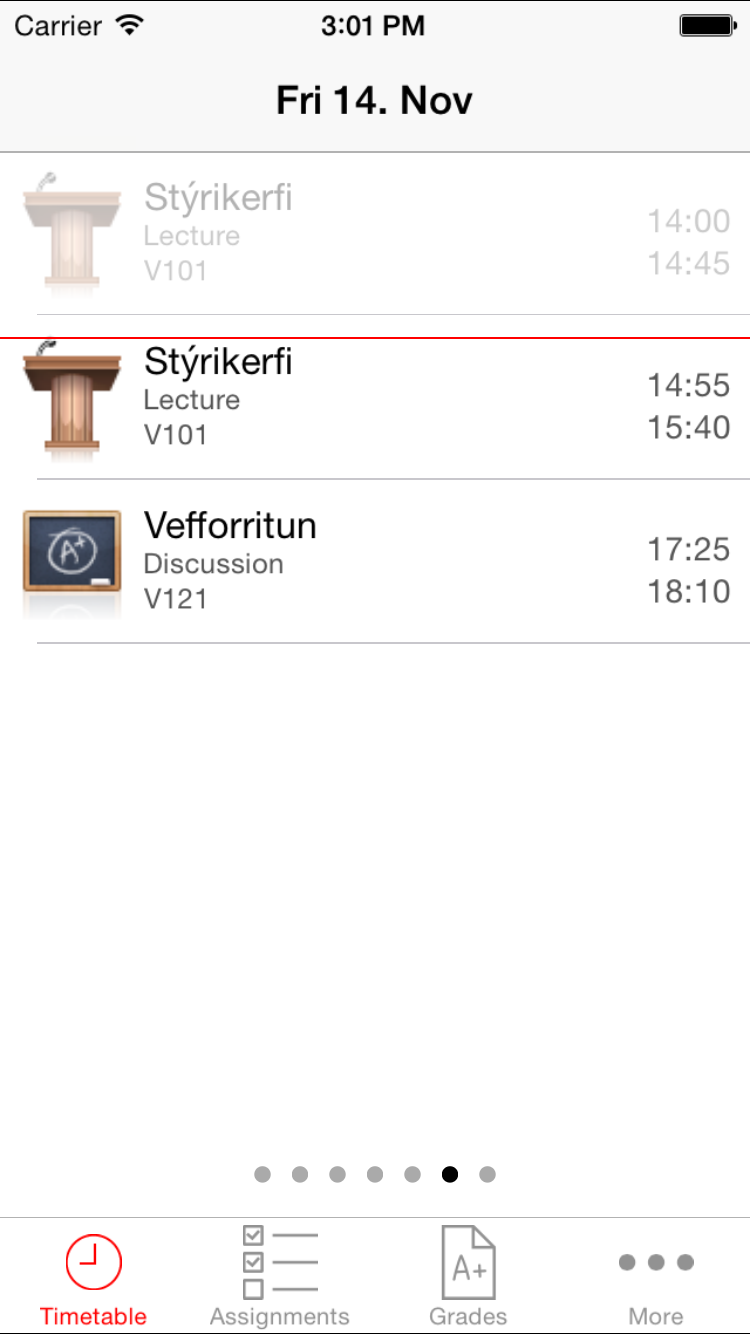
\includegraphics[width=0.45\textwidth]{schedule.png}
    \hspace{0.2in}
    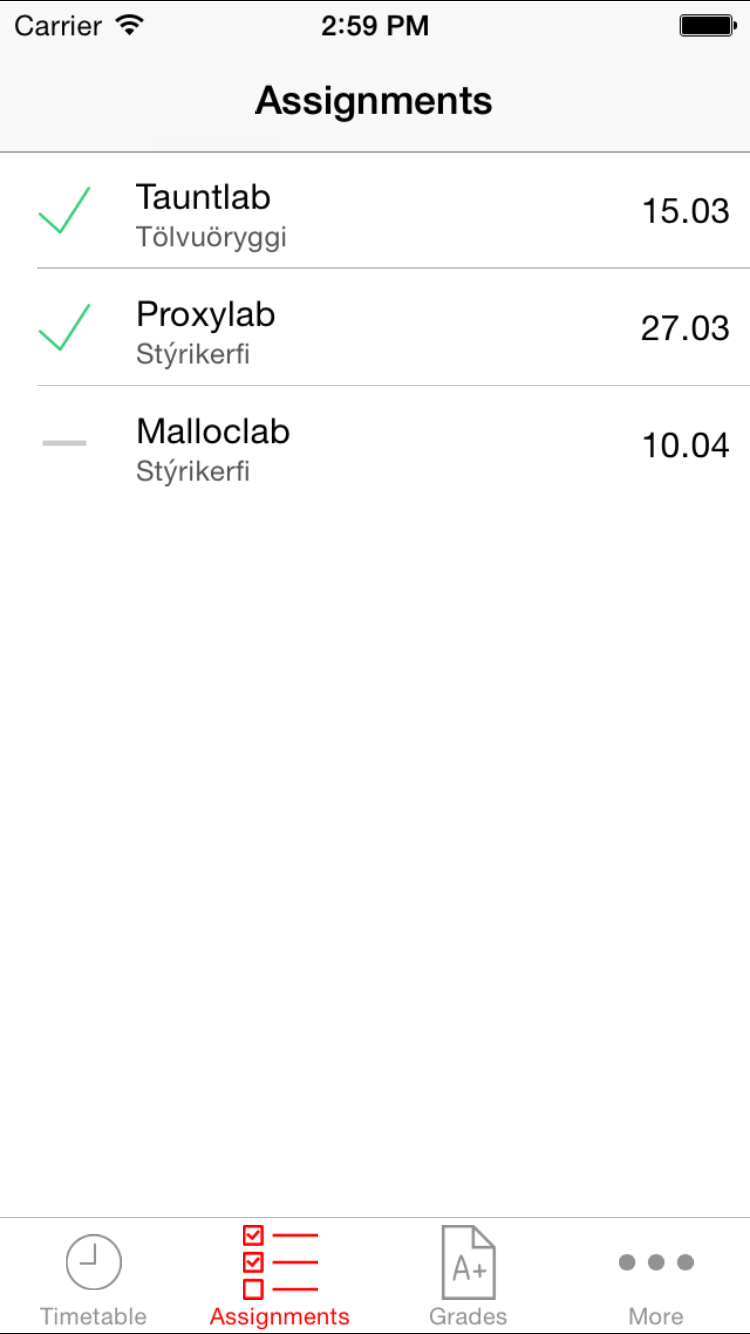
\includegraphics[width=0.45\textwidth]{assignments.png}
    \caption{Schedule and assignments.}
    \label{fig:grades}
\end{figure}

\subsection{Schedule}

This tab in the application displays a user's upcoming classes, when they start, in what room they
take place and what sort of class it is. We display the data in a table, and a moving red line indicates
how far in to the current class a user is. One can swipe left or right to examine schedule for
the surrounding days as well. This functionality has been significantly improved from MyRU,
where it was only possible to view the schedule for the current day.

\subsection{Assignments}

One of the most important features a mobile client must include is viewing upcoming assignments.
The assignments tab presents a list of due assignments, along with the due date for each and a check-mark
indicating whether it has been handed in. If a user selects an assignment from the list, he or she
is presented with a view containing the MySchool page for that assignment, and will be able to hand
it in or mark it as such from within the app with a single tap. The assignment details page contains
data that is infeasible to parse, so we choose to render the MySchool page within a web view. Ideally
we would define our own UI for presenting this information but that is not feasible with the current
situation. If MySchool were to have an API this situation would be very different and we would be
able to provide our users the complete experience they really want.

\subsection{Grades}

\begin{figure}[t]
    \centering
    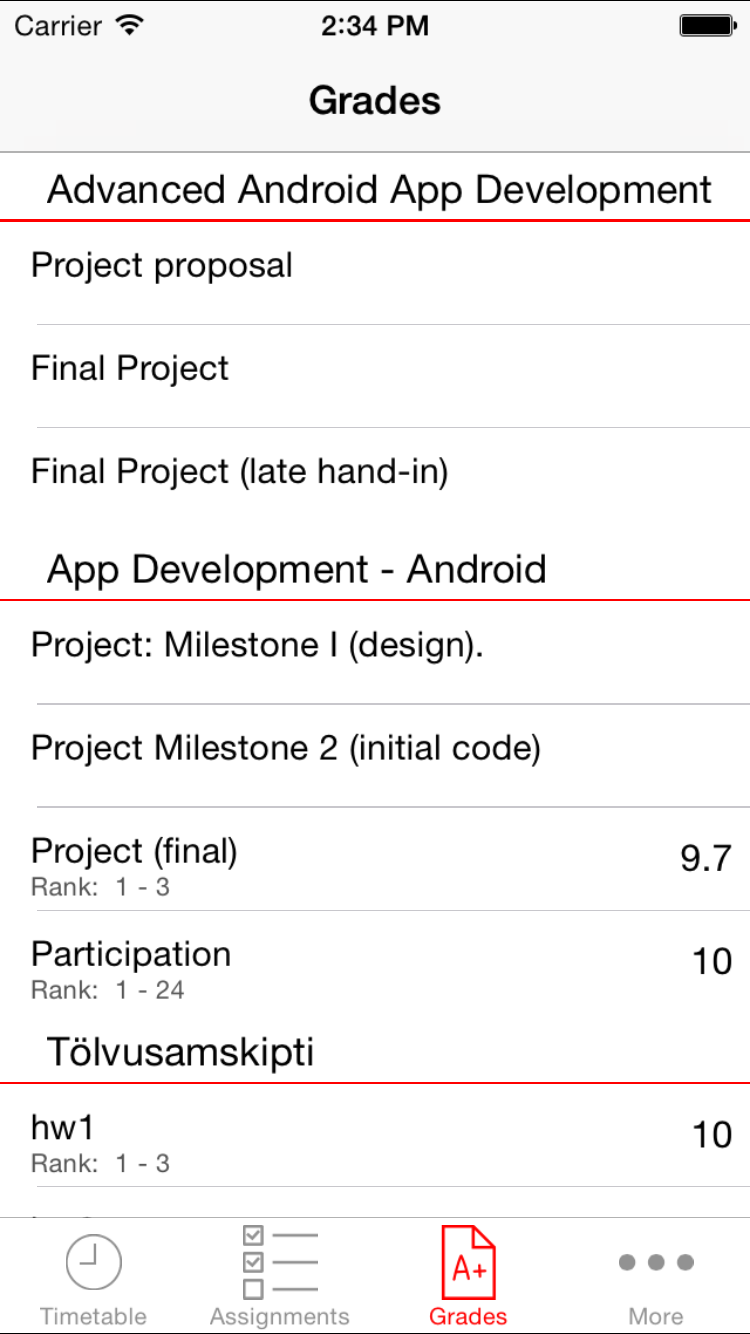
\includegraphics[width=0.45\textwidth]{grades.png}
    \hspace{0.2in}
    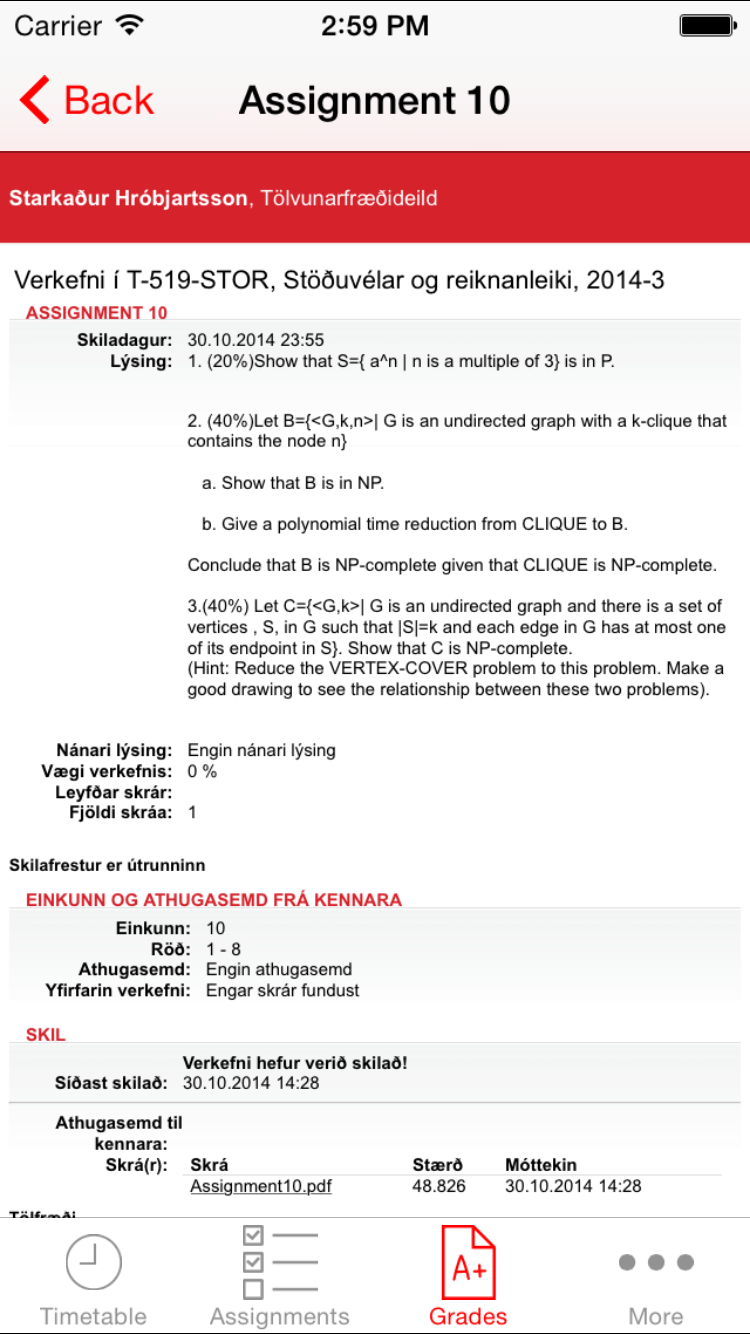
\includegraphics[width=0.45\textwidth]{grades-detail.png}
    \caption{The grades view and corresponding detail view.}
    \label{fig:grades}
\end{figure}

Grades are presented in an analogous manner to the assignments, with a web view shown once a 
user selects a grade. 

\subsection{More}

In the "more" tab a user can view the week's menu in Málið and log out.
This menu will come to contain more functionality in the future, but currently it's limited to the items mentioned
above. In section \ref{sec:future} we will discuss in detail many of the other features the app 
could have, but to mention one that would be relevant to this section we planned to implement
MySchool's phonebook lookup feature in the app and place it under the More tab. Unfortunately this, as
many other ideas, proved infeasible without a proper API.

%------------------------------------------------


\section{Architecture}
\label{sec:arch}

The app design follows the MVC (Model View Controller) pattern encouraged by Apple in iOS development.
The principles are that model classes are wrappers for data and contain methods to manipulate that
data, views are classes that own UI components and know how and when to render them to the screen
and controllers are the interface between the two. They listen for events and react appropriately, 
fetching data from a model and giving it to a view, or transition between views.

Classes are written to be loosely coupled, ensuring that changing one part of the application, such 
as the parser, will not affect other components. This ensures maintainability and robustness to
changes in the way we interact with MySchool.

We use external libraries for XML parsing and network communication. These external dependencies 
are managed through Cocoapods\cite{pods}, a dependency management tool for iOS and OS X development.
This tool fetches the libraries and adds a build phase to link it. Since most
external libraries out there are written in Objective-C we added a bridging header to interface
with them. The compiler then automatically generates a Swift interface and casts return types to 
proper Swift types. This is a fantastic feature of Swift mentioned briefly above, and really eases
the transition over to Swift.

The app involves three separate targets. iOS 8 introduces so called app-extensions\cite{extensions}. This is an extension
of the app sandbox that allows a separate process to share data with the main application. We use
this to implement a Today-view extension, a plugin for the iOS Today-view that shows upcoming classes
and assignments at a glance. In order to share common code between the app and the extension we
create a framework called \texttt{iSchool.framework} that contains all the shared logic. In this 
section we describe the design of each of the three targets.

\subsection{Framework}
The framework target contains the components that need to be shared between the app and the extension.
This includes the various model classes and components to handle parsing, authentication, credential
management and data storage.

Having all of this shared code in a framework makes future work easier. For example a desktop Mac
application could be created with minimal work by linking with the framework. This also simplifies
maintenance work as changes affecting both the app and the extension need only be made in one place.

\subsection{App}

\begin{figure}
    \centering
    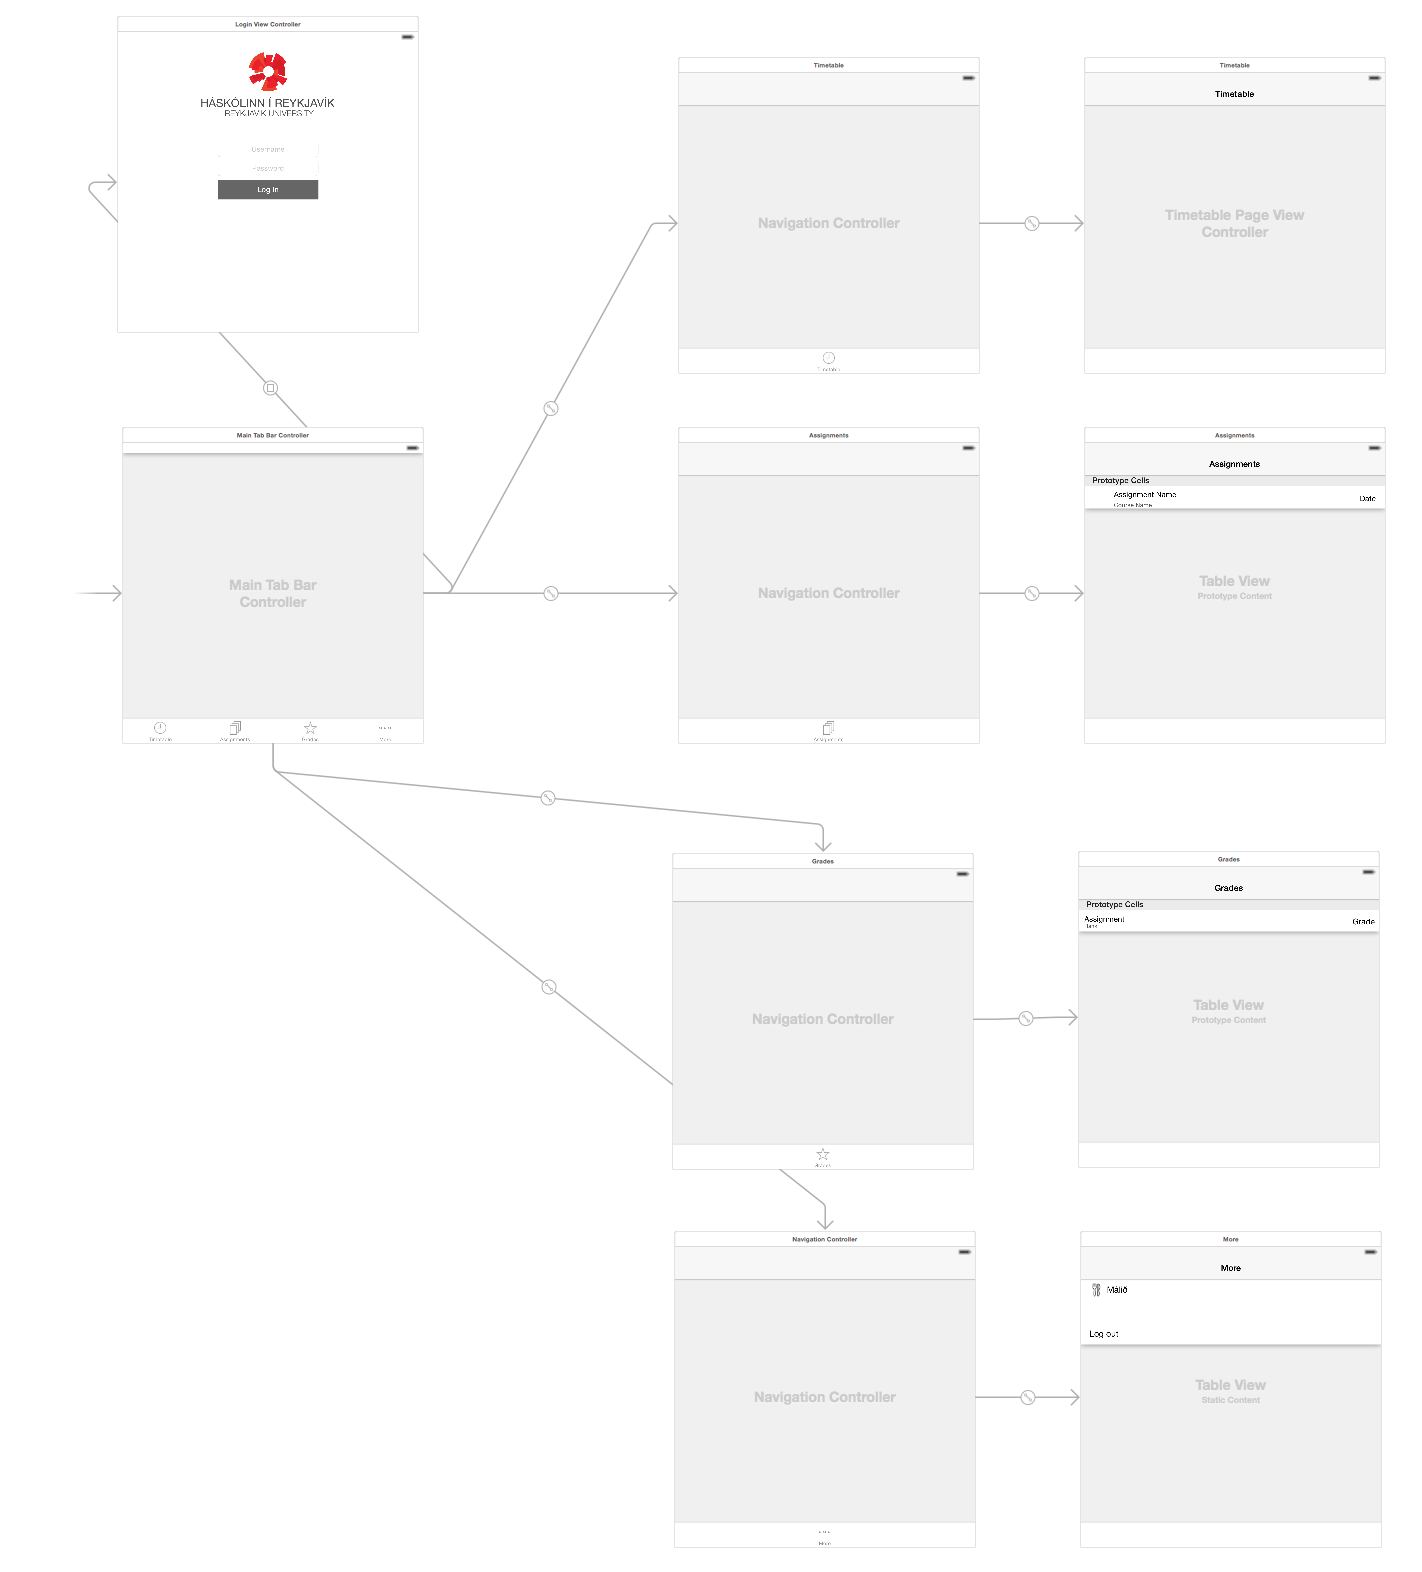
\includegraphics[width=0.45\textwidth]{view-tree.png}
    \caption{A diagram showing the relationship between views (simplified)}
    \label{fig:hierarchy}
\end{figure}

The app target includes all the views and controllers for the various UI components. 
The main design concern with the app is the view controller hierarchy. The first view the app 
presents when it opens is called the root view. It then has other views as subviews and so forth
creating a tree of views. The way we design this tree is by having the tab bar at the root of the
tree, and it's subviews as navigation views. Each of the navigation views then has several subviews
of it's own for each tab. Figure \ref{fig:hierarchy} shows the relationship between the views
graphically.

One of the main problems with MyRU was concurrency. We were doing a lot of computation on 
the main thread, causing the UI to lock up. To solve this in the new app we have one thread for 
network communication, and one for processing. When data is ready to be displayed that thread sends
a message to the UI thread indicating that new data is available, or that an error occurred. The UI
then reacts appropriately while staying responsive the whole time. Controllers register themselves 
to receive a notification, so more than one controller can react to the same message. iOS makes this
very easy with the notification center API.

To summarize, we tried our best to ensure separation of concerns and avoid code duplication as much
as possible. This ensures the app will be maintainable in the future.

\subsection{Extension}

\begin{figure}
    \centering
    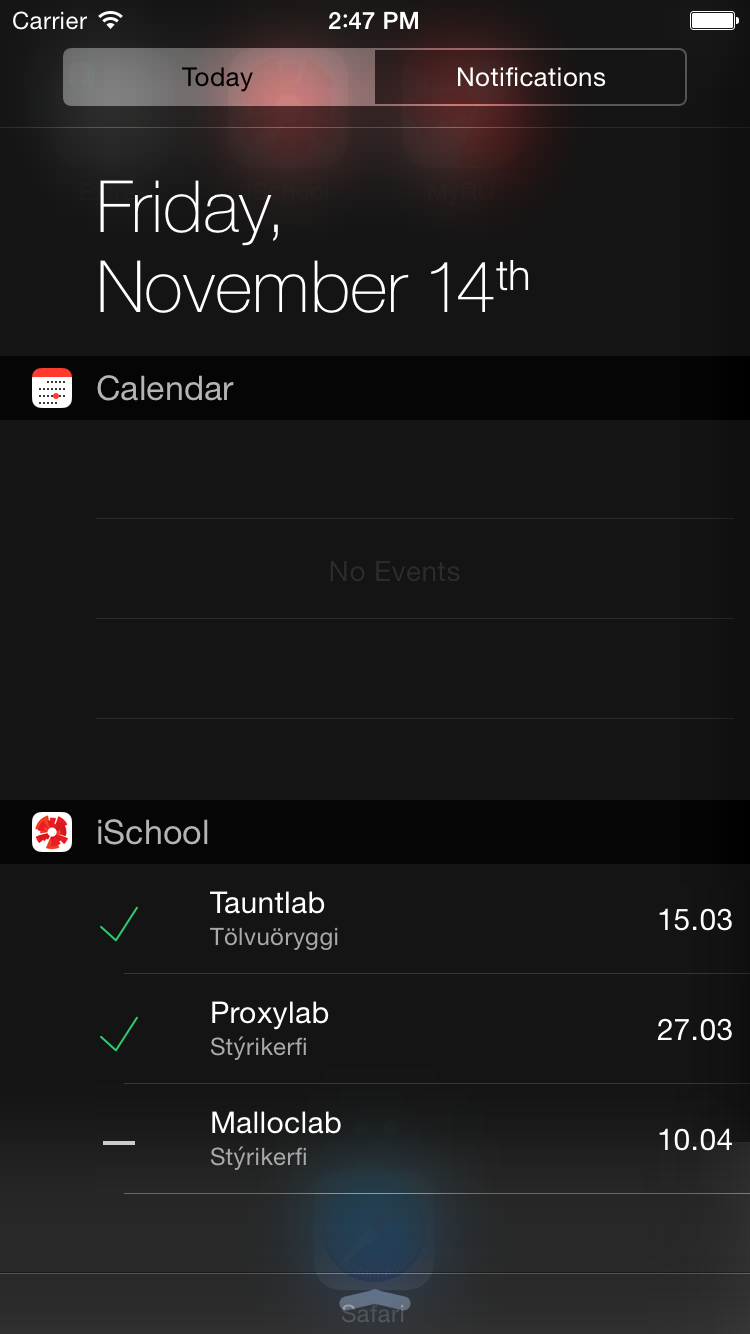
\includegraphics[width=0.25\textwidth]{widget.png}
    \caption{The Today-view with the iSchool extension}
    \label{fig:today}
\end{figure}

The extension consists of a single view and a corresponding controller. It communicates with the
main app for data and renders it in a table in the Today view. It links against the framework for 
credential management and communication with MySchool. Figure \ref{fig:today} shows what the
extension looks like in the Today-view.

%--------------------------------------------------------------------
%   Progress Section
%--------------------------------------------------------------------

\section{Progress}
\label{sec:progress}

Work began on the app on August 28. We began by creating a backlog of tasks, maintained online in
Trello\cite{trello}. We conducted requirements analysis to determine which features are appropriate and broke
them down into actionable tasks so we could
have an overview of the development progress. Learning the Swift language was easy, as the syntax
is familiar, and we were able to get started quickly and overcome issues as the cropped up.
The development went smoothly for the most part, although we ran into some trouble due to API changes as discussed in section \ref{sec:swift}.
As the language is very new, online documentation was lacking on many details
and we were left to fend for ourselves in a lot of 
cases. This did not cause significant problems and we managed to overcome all hurdles we encountered.

We used the open source version control system git for source control and all code is stored in an open Github\cite{github} repository and made available
to the public as a open source project under a BSD license\cite{licence}. Anyone is free to examine the source
and use components in their own work or contribute improvements.

Work progressed according to the absolute-value sine-wave model, which I believe we pioneered. This 
involves doing nothing for extended periods and then suddenly doing a lot of work at once. Due to 
other courses interfering with the work from time to time this development model was deemed 
appropriate.

We left most of the UI design up to the last minute, preferring to focus initially on the app logic
and designing the interface when we had a better idea of what the finished product would look like.

We had to scrap a few ideas that we wanted to include initially due to limitations of how MySchool
presents some data.

Development continued until November 14, when the app was ready for the App Store.
Our initial estimate was that we would spend approximately 400 hours on the project, based on the
number of ECTS credits. Learning Swift took less time than anticipated, and since we had a good idea
of what needed to be done and some previous experience we were able to finish the app with around
300 hours of development time. This includes dealing with the aforementioned difficulties with Swift
and the initial time investment of writing proper tests, although this payed dividends at the end.
The effort we put in was divided evenly among us, and we were quite pleased with how well it went.

%--------------------------------------------------------------------
%   Progress Section
%--------------------------------------------------------------------

\section{Future work}
\label{sec:future}

We believe this project presents a lot of potential for further development. If MySchool were to
present an API in the future the functionality of the app could be significantly extended.

Significant work has been done on an API by Centris\cite{centris}, an organisation associated with
Reykjavik University including both students and staff at the university. When it's ready for deployment it will open
up a world of possibilities, both for our app and other applications, such as a more modern web 
interface.

Some of the ideas that we wanted to include but deemed infeasible or impractical due to the absence
of an API were:

\begin{itemize}
    \item View upcoming events such as "Science trips" and online exams.
    \item Push notifications for upcoming events.
    \item Statistics and historical overview of grades in previous courses.
    \item Sign up for events through MySchool
    \item Redeem print codes through \texttt{hrprint.ru.is}.
    \item Look up students and staff in the MySchool phonebook.
    \item Toggle reminders on specific classes.
\end{itemize}

We consider further work on the app to be a good potential project for other students wishing to 
familiarize themselves with iOS app development and those interested in potentially improving the
lives of their fellow students. 

Due to the fact that the application has been designed from the start with reusability and modularity
in mind, a minimal time investment would be required to adapt the app to other systems with similar
purpose, for example the University of Iceland intranet, Uglan\cite{uglan}.

\section{Conclusion}

In this report we have explained the problems students face when accessing MySchool on a mobile 
device. The solution we proposed was a native iOS application that presents the most relevant 
MySchool functionality in an easy to use, intuitive format. We gave an outline of the design of the
app, explained various design decisions and the reasoning behind them. We also gave a short overview
of the new programming language Swift, and how the choice to use it factored into the development 
process.

As we have shown in section \ref{sec:myru}, there is great interest in an app to simplify accessing
MySchool from a mobile client. This leads us to believe that the new application we have
developed for this project will be popular among students of the university, and significantly
enhance their interaction with MySchool. We realise that user experience matters a great deal and
can greatly influence perceived value. In light of this fact we are certain that students will be pleased
when given a simple tool to interact with this very important part of a RU students life. 
The entire educational experience becomes more pleasant when we have good tools to interact with, and 
students will receive greater value from their studies.

\pagebreak

%----------------------------------------------------------------------------------------
%	REFERENCE LIST
%----------------------------------------------------------------------------------------

\begin{thebibliography}{9}

\bibitem{myschool} 
    \url{http://myschool.ru.is/myschool}

\bibitem{RU statistics} 
    \url{http://www.ru.is/haskolinn/tolfraedi/nemendur-i-hr/}

\bibitem{myru} 
    \url{https://itunes.apple.com/is/app/myru/id793259120?mt=8}

\bibitem{ios} 
    \url{http://www.apple.com/ios/}

\bibitem{swift} 
    \url{https://developer.apple.com/swift/}

\bibitem{android} 
    \url{http://www.google.com/mobile/android/}
    
\bibitem{wwdc} 
    \url{https://developer.apple.com/wwdc/}

\bibitem{llvm} 
    \url{http://llvm.org}

\bibitem{pods} 
    \url{http://cocoapods.org}

\bibitem{github} 
    \url{http://www.github.com}

\bibitem{license} 
    \url{http://opensource.org/licenses/BSD-2-Clause}

\bibitem{extensions} 
    \url{https://developer.apple.com/app-extensions/}

\bibitem{centris} 
    \url{https://bitbucket.org/ru_scs/centrisapi}

\bibitem{uglan} 
    \url{https://ugla.hi.is}

\end{thebibliography}

%----------------------------------------------------------------------------------------

\end{document}
